For at facilitere nem adgangen til databasen med hensyn til 
opsætning af kasseapparatet er der lavet et \gls{WebAPI}. 
Det hele er lidt en to delt affære den ene del er implementeringen af et \gls{RESTful} API,
Den anden er implementeringen af en web grænseflade som bruger \gls{RESTful} API'en til at lave ''Create, Read, Update og Delete'' i databasen.

\subsubsection{RESTful}
Et \gls{RESTful} API som betyder \gls{REST} det bruges over \gls{HTTP} med xml eller json til at repræsentere objekter.
Her kan bruges \gls{HTTP} verber sammen med \gls{URI}.
Der kan således skrives ''GET /api/products'' herved vil man få en liste af produkter.

\begin{figure}[H]
    \centering
	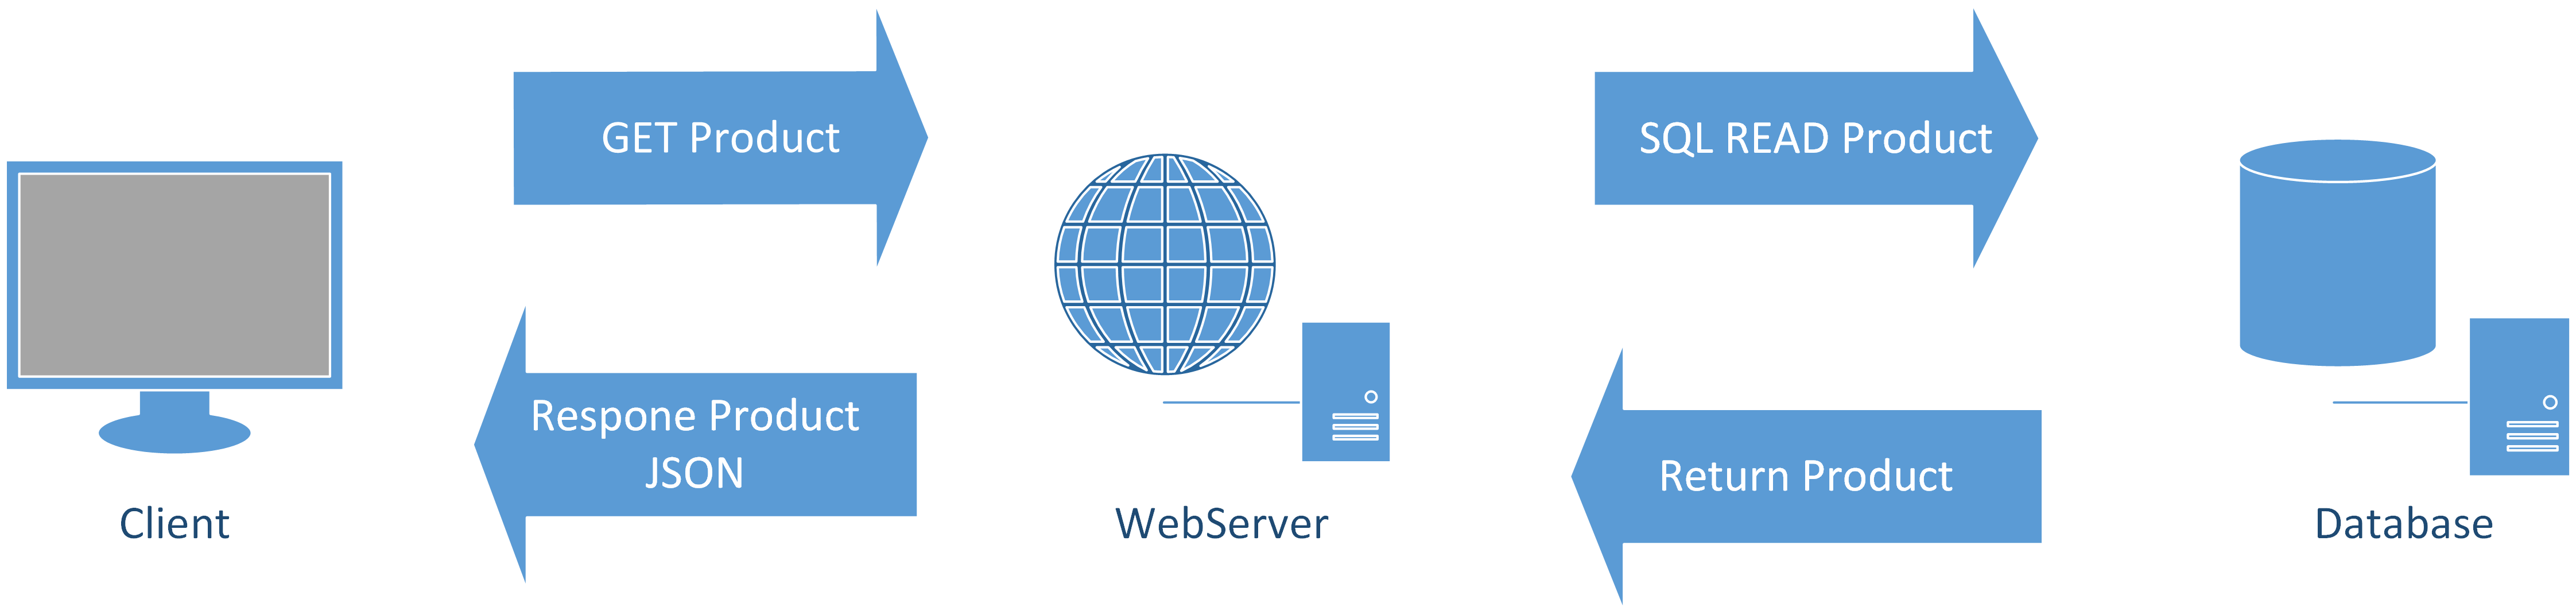
\includegraphics[scale=0.8]{Rapport/RESTful.PNG}
	\caption{RESTful API}
	\label{fig:RESTfulApi}
\end{figure} 

Alt dette gør at det er nemt at tilgå data igennem vores webserver som det er illustreret i figur \ref{fig:RESTfulApi}.
Der kan udover ''GET'' også bruges ''PUT'', ''POST'' og ''DELETE''. 

\subsubsection{Web Interface}
Til at bruge \gls{RESTful} API'en er der lavet et web interface i \gls{ASPNET} som gør brug af \gls{MVC} mønsteret.

\begin{figure}[H]
    \centering
	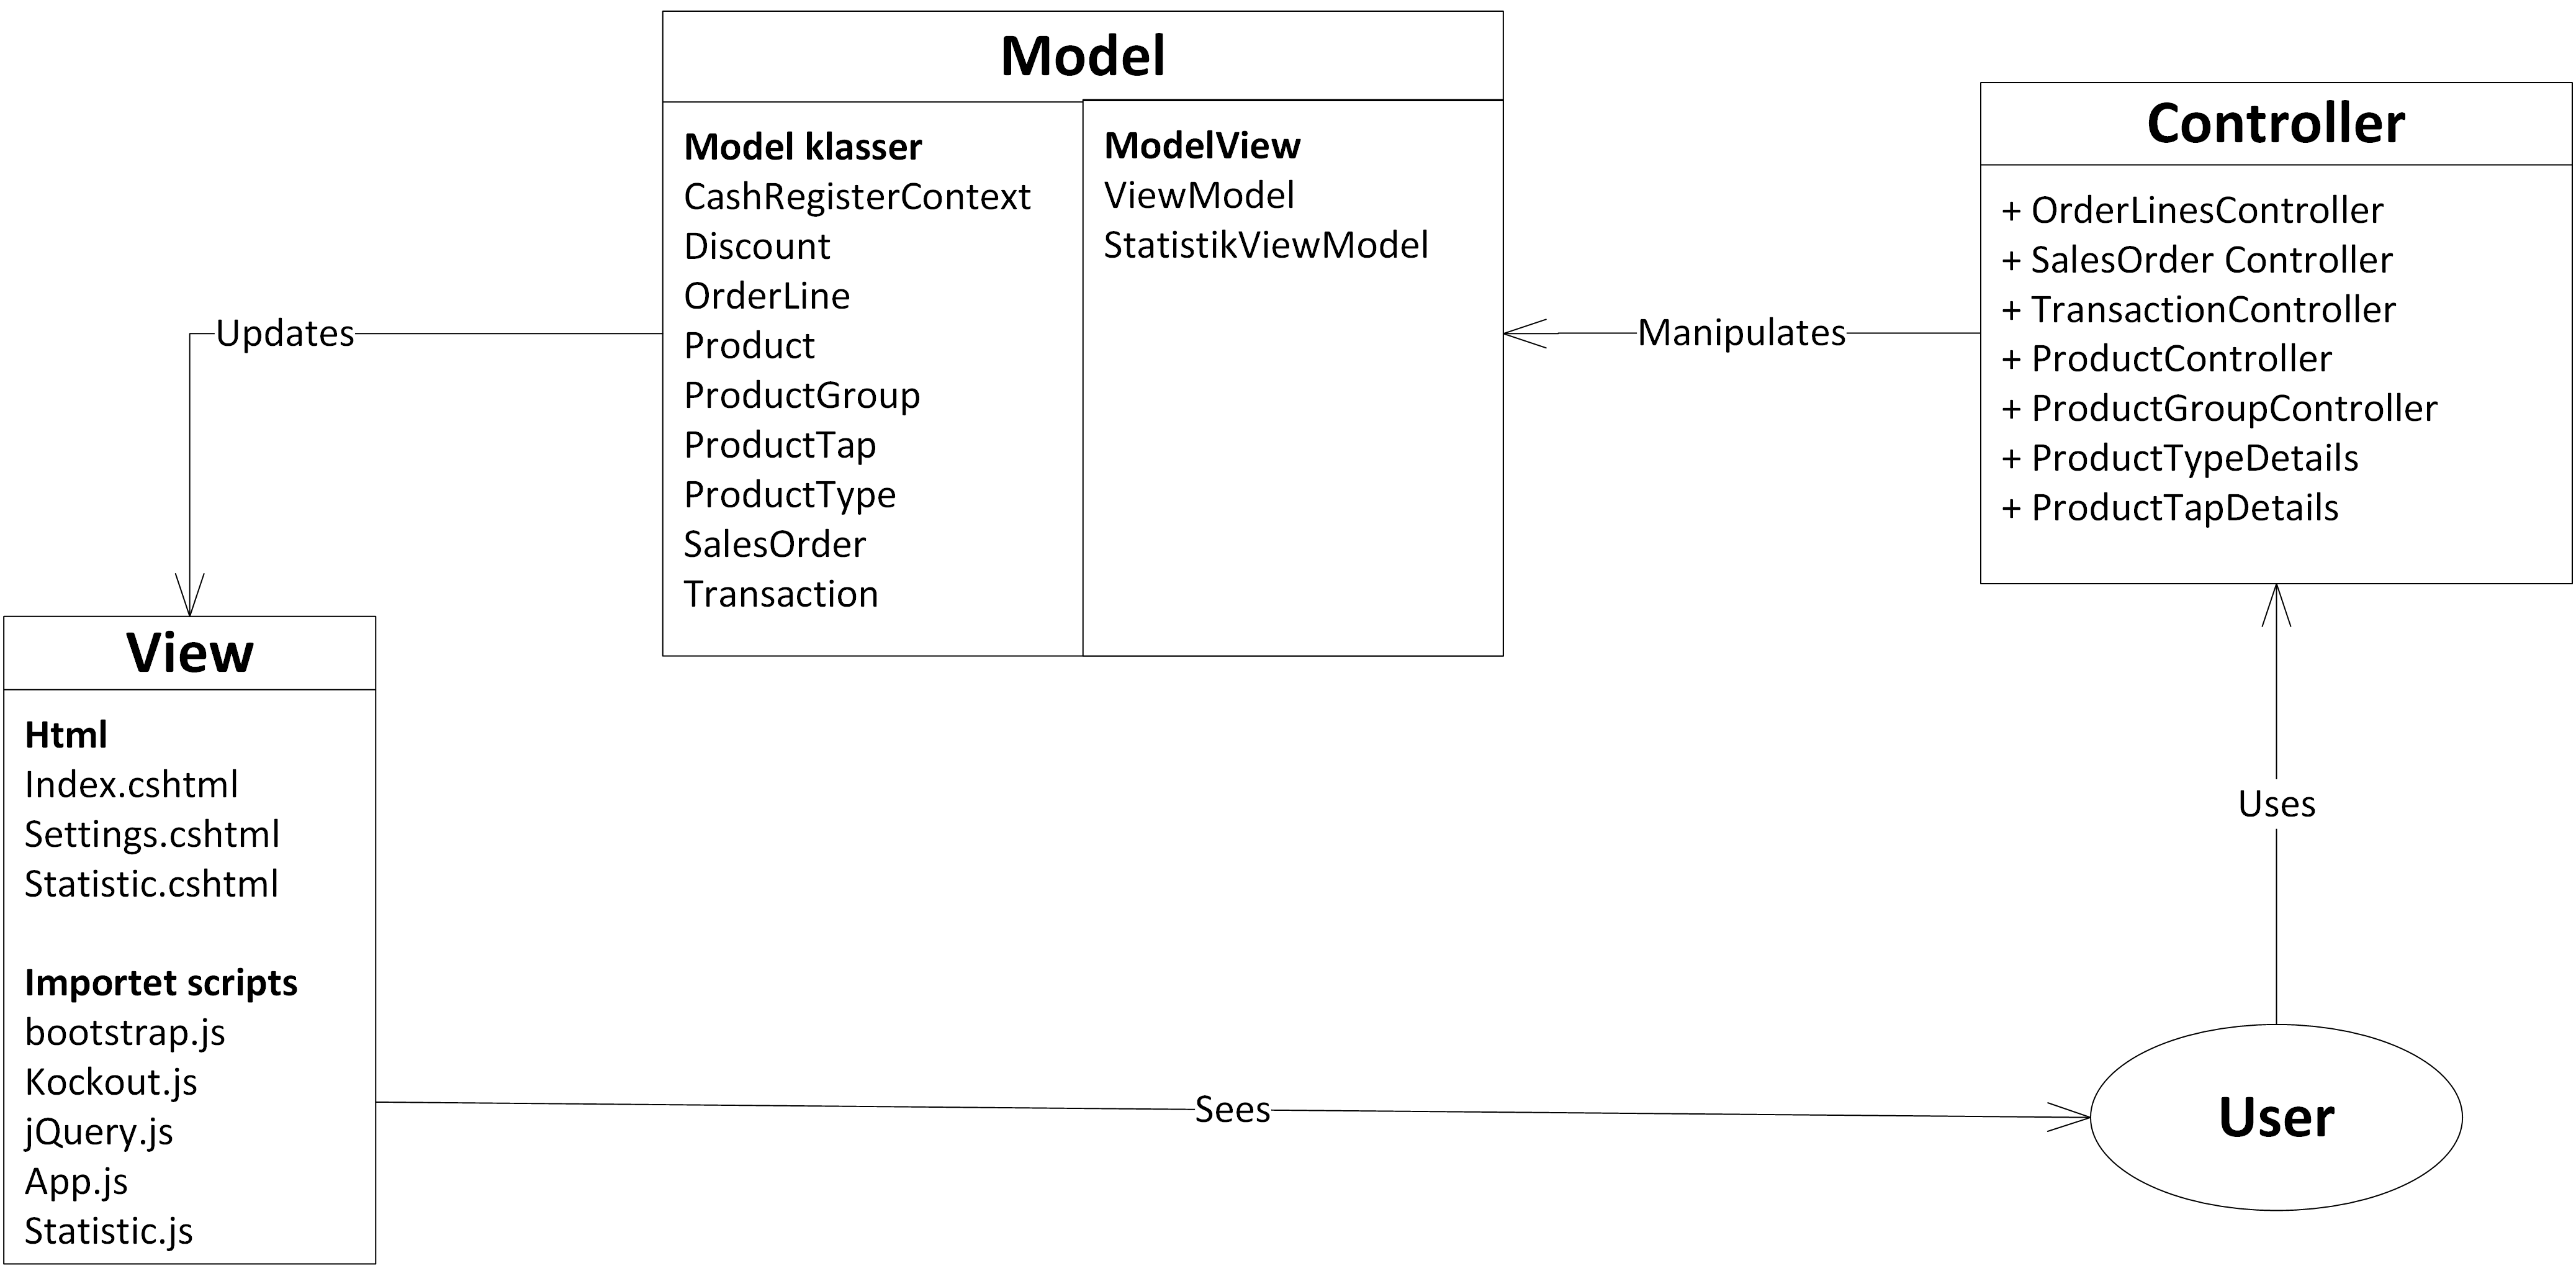
\includegraphics[scale=0.8]{N+1/LogicalView/WebApi/WebView/WebViewDiagram.png}
	\caption{MVC i cash registers web interface}
	\label{fig:MVCWebApi}
\end{figure} 

I figur \ref{fig:MVCWebApi} kan opbygning af web interfacet ses. 
Der er blevet brugt en kombination af javascript, CSS og html til at konstruere interfacet som udgør view delen.
I javascript delen er der brugt en del biblioteker som bootstrap til opsætning af interfacet, knockout til at lave views der er responsive og jQuery.
Model delen er de klasser der er stillet op for produkter med videre. 
Controllerne er der hvor \gls{REST} er implementeret.

